\documentclass[a4paper,11pt]{report}

%%%%%%%%%%%%%%%%%%%%%%%%%%%%%%%%%%%%%%%%%%%%%%%%%%%%%%%%%%%%%%%%%%%%%%%
% Definicion de paquetes
\usepackage[T1]{fontenc}
\usepackage[spanish]{babel}
\usepackage{xargs}                      % Use more than one optional parameter in a new commands
\usepackage[pdftex,dvipsnames]{xcolor}  % Coloured text etc.

%%%%%%%%%%%%%%%%%%%%%%%%%%%%%%%%%%%%%%%%%%%%%%%%%%%%%%%%%%%%%%%%%%%%%%%
% Definición de comandos
\usepackage[colorinlistoftodos,prependcaption,textsize=tiny]{todonotes}
\newcommandx{\unsure}[2][1=]{\todo[linecolor=red,backgroundcolor=red!25,bordercolor=red,#1]{#2}}
\newcommandx{\change}[2][1=]{\todo[linecolor=blue,backgroundcolor=blue!25,bordercolor=blue,#1]{#2}}
\newcommandx{\info}[2][1=]{\todo[linecolor=OliveGreen,backgroundcolor=OliveGreen!25,bordercolor=OliveGreen,#1]{#2}}
\newcommandx{\improvement}[2][1=]{\todo[linecolor=Plum,backgroundcolor=Plum!25,bordercolor=Plum,#1]{#2}}
\newcommandx{\thiswillnotshow}[2][1=]{\todo[disable,#1]{#2}}

%%%%%%%%%%%%%%%%%%%%%%%%%%%%%%%%%%%%%%%%%%%%%%%%%%%%%%%%%%%%%%%%%%%%%%%
%% Empieza el documento
\begin{document}
\title{Identificación de riesgos}
\author{
		Sergio García Sánchez
		\and
		Sara Juberías Campos
		\and
		José Luis Mela Navarro
		\and
		Amalia Regueira Fernández
		\and
		Miguel Emilio Ruiz Nieto
	}

\maketitle
\section*{Identificación de riesgos}

Para hacer una identificación de los posibles riesgos que puedan surgir en la realización
de este proyecto nos hemos ayudado de la matriz de riesgos como herramienta de gestión, haciendo un análisis objetivo de las funcionalidades que hay que desarrollar.

\begin{figure}[h]
    \centering
    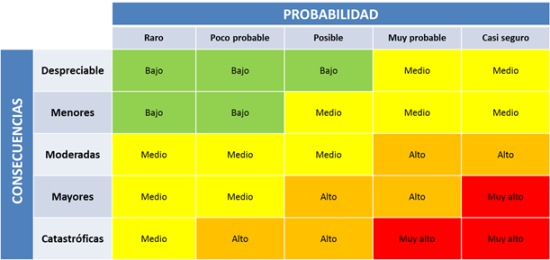
\includegraphics[height=5cm, width=12cm]{matriz_riesgos.png}
    \caption{Matriz de riesgos}
\end{figure}

Así pues, los riesgos identificados para el desarrollo de este proyecto son:

\begin{itemize}
    \item Diseño de interfaz. No está acordado un diseño específico de interfaz
    con el cliente, por tanto es casi seguro que exista este riesgo. Por ello,
    lo clasificamos como muy alto.
    % (No está definida con el cliente, probabilidad: casi seguro, consecuencias: mayores, riesgo: muy alto)
    \begin{itemize}
        \item Plan de contingencia: definir la interfaz con el cliente.
        \item Plan de atenuación: Estudiar con el cliente qué cambios se pueden
        realizar en la interfaz existente.
    \end{itemize}

    \item Falta de diseñadores: No se ha contemplado que uno de los
    desarrolladores sea especialista en diseño de interfaces de usuario, así que
    contamos con la experiencia que puedan tener los desarrolladores senior y
    junior. Este riesgo está relacionado con el anterior, dando lugar a que con
    casi toda certeza pueda darse este riesgo. Así pues, también consideramos
    este riesgo como muy alto.
    %  (No está contemplado en el personal una persona especializada en UX, probabilidad: casi seguro, consecuencias: mayores, riesgo: muy alto)
    \begin{itemize}
        \item Plan de contingencia: Formar a un miembro del equipo de desarrollo
        como diseñador UX.
        \item Plan de atenuación: Contratar a un miembro del equipo de
        desarrollo como diseñador UX.
    \end{itemize}

    \item Implementación nuevas funcionalidades: Existe la posibilidad de que
    el cliente pida nuevas funcionalidades para la aplicación requerida. A pesar
    de que en el contrato firmado con el mismo hay una claúsula en la cual se
    indica que asumimos las posibles nuevas funcionalidades que se requieran
    siempre y cuando ambas partes estén de acuerdo, concluimos que puede existir
    un riesgo medio de darse este caso.
    % (probabilidad: probable, consecuencias: moderado, riesgo: medio)
    \begin{itemize}
        \item Plan de contingencia: Subcontratar una empresa para realizar
        las nuevas funcionalidades.
        \item Plan de atenuación: Reunirse con el cliente para redefinir los
        plazos de entrega.
    \end{itemize}

    \item Calidad empresa subcontratada: Nuevamente, existe una cláusula en el
    contrato con el cliente en la cual se especifica que nosotros, como
    desarrolladores, podemos contratar una empresa subcontratada para delegar
    nuestros servicios, siendo nuestro equipo el responsable directo de los
    perjuicios que dicha empresa pueda ocasionar. Consideramos como poco
    probable este riesgo dado que en nuestra planificación no está contemplado
    el hecho de subcontratar algún servicio, por lo tanto el riesgo para este
    punto sería bajo.
    %   (probabilidad: poco probable, consecuencias: menores, riesgo: bajo)
    \begin{itemize}
        \item Plan de contingencia: Buscar la mejor compañía que se ajuste al
        presupuesto de las funcionalidades que puedan surgir.
        \item Plan de atenuación: Enviar un miembro del equipo a supervisar
        que dichas funcionalidades se estén implementando correctamente.
    \end{itemize}

    \item Baja productividad: Consideramos como muy probable este riesgo dado
    que es nuestro primer proyecto como desarrolladores y no conocemos bien a
    todos los integrantes del equipo. Las consecuencias de dicho riesgo serían
    moderadas y el riesgo, por tanto, sería alto.
    %  (probabilidad: muy problable, consecuencias: moderadas, riesgo: alto)
    \begin{itemize}
        \item Plan de contingencia: Lograr que el ambiente de trabajo sea
        agradable.
        \item Plan de atenuación: Hablar con el personal afectado para acordar
        una solución.
    \end{itemize}

    \item Requisitos demasiado complejos: A priori este riesgo no está
    contemplado como que pueda ocurrir dado que nuestro presupuesto está
    ajustado a la complejidad que hemos considerado de las funcionalidades.
    Así que, a pesar de que este riesgo es raro que suceda, sus consecuencias
    son mayores pero su riesgo es medio.
    %   (probabilidad: rara, consecuencias: mayores, riesgo: medio)
    \begin{itemize}
        \item Plan de contingencia: Revisar la especificación de funcionalidades
        acordadas con cliente. Formación del equipo de desarrollo.
        \item Plan de atenuación: Renegociar los plazos de entrega con el
        cliente.
    \end{itemize}

    \item Conocimientos del equipo: Como hemos comentado anteriormente, nuestro
    equipo no cuenta en proyectos anteriores de esta envergadura, luego es
    muy probable que tengamos un riesgo de estas características, dando lugar
    a consecuencias catastróficas que puedan dificultar que cumplamos los plazos.
    %   (probabilidad: muy probable, consecuencias: catastróficas, riesgo: alto)
    \begin{itemize}
        \item Plan de contingencia: Formación del equipo impactado.
        Revisiones más periódicas.
        \item Plan de atenuación: Reemplazar al miembro del equipo si se
        considera que la formación no ha sido suficiente.
    \end{itemize}

\end{itemize}
\end{document}